% 真空中的平面电磁波
% 麦克斯韦方程组|电磁波|平面波|波动方程

\pentry{麦克斯韦方程组\upref{MWEq}}

\begin{figure}[ht]
\centering
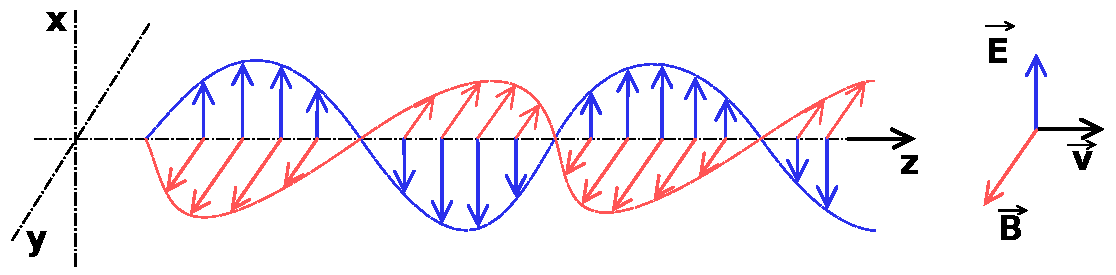
\includegraphics[width=9cm]{./figures/VcPlWv_1.pdf}
\caption{平面电磁波的电磁场分布. 注意于电磁场矢量与 $x, y$ 坐标无关, 并占据整个空间(图片来自维基百科)} \label{VcPlWv_fig1}
\end{figure}

\footnote{参考 \cite{GriffE} 相关章节.}平面电磁波如\autoref{VcPlWv_fig1} 所示. 电场与磁感应强度的关系为
\begin{equation}
\abs{B(\bvec r)} = \abs{E(\bvec r)}/c
\end{equation}
平均能流密度(光强)为(推导见\autoref{EBS_ex1}~\upref{EBS})
\begin{equation}
I = \frac12 c\varepsilon_0 E_0^2
\end{equation}
波速等于真空中的光速 $c$, 且
\begin{equation}\label{VcPlWv_eq1}
c = \frac{1}{\sqrt{\epsilon_0\mu_0}} = 299,792,458 \Si{m/s}
\end{equation}

\subsection{推导}
(描述未完成)

\begin{equation}
\curl(\curl \bvec E) = -\curl\pdv{\bvec B}{t} = -\epsilon_0\mu_0 \pdv[2]{\bvec E}{t}
\end{equation}

\begin{equation}
\curl(\curl \bvec E) = \grad(\div \bvec E) - \laplacian \bvec E = - \laplacian \bvec E
\end{equation}

\begin{equation}
\laplacian E = \epsilon_0 \mu_0 \pdv[2]{\bvec E}{t}
\end{equation}

\begin{equation}
E_y = E_0\cos(\omega t - kx)
\end{equation}
